\documentclass[11pt]{article}
\usepackage{acl}
\usepackage{times}
\usepackage{latexsym}
\usepackage{fontspec}
\usepackage{graphicx}
\usepackage{booktabs}
\usepackage{amssymb}
\usepackage{amsmath}
\usepackage{multirow}
\usepackage{hyperref}

\setmainfont{Times New Roman}

\title{Đánh Giá Hiệu Quả Các Phương Pháp Khuyến Nghị Truyền Thống và Học Sâu trên Dữ Liệu Tương Tác Người Dùng--Món Ăn từ Nền Tảng Ẩm Thực Trực Tuyến Việt Nam}

\author{
  Sinh viên Thực hiện \\
  Khoa Khoa học và Kỹ thuật Thông tin \\
  Trường Đại học Công nghệ Thông tin, ĐHQG-HCM \\
  \texttt{\{sinhvien\}@gm.uit.edu.vn}
}

\date{}

\begin{document}
\maketitle

\begin{abstract}
Trên các nền tảng ẩm thực trực tuyến, hành vi đánh giá món ăn (rating) tạo thành dữ liệu tương tác người dùng có giá trị cho bài toán khai thác sở thích cá nhân. Nghiên cứu này sử dụng bộ dữ liệu ViFoodRec \cite{tran2024vifoodrec}---182.678 lượt tương tác người dùng--món ăn thu thập từ cộng đồng ẩm thực Việt Nam---để đánh giá thực nghiệm \textbf{bốn họ phương pháp khuyến nghị}: Content-Based Filtering (CBF), Memory-Based Collaborative Filtering (CF), Funk SVD và Neural Collaborative Filtering (NCF). Ba câu hỏi nghiên cứu được đặt ra: (RQ1) hiệu quả của CBF và CF trên dữ liệu tương tác MXH ẩm thực Việt; (RQ2) liệu Matrix Factorization và NCF có cải thiện dự đoán rating so với phương pháp truyền thống; (RQ3) mô hình nào phù hợp hơn cho Rating Prediction và Top-$K$ Recommendation. Kết quả cho thấy NCF giảm RMSE xuống 1.5898 (thấp hơn User-CF 3.2\%), trong khi User-CF (Cosine) đạt Precision@10 cao nhất (39.50\%) dù chênh lệch giữa các mô hình ranking chỉ khoảng 1--2 điểm phần trăm. Nghiên cứu phân tích ý nghĩa thống kê, hạn chế và nguồn lỗi trên dữ liệu tương tác xã hội.
\end{abstract}

% ============================================================
\section{Giới thiệu}
\label{sec:intro}
% ============================================================

\subsection{Bối cảnh: Khai thác dữ liệu tương tác trên nền tảng ẩm thực trực tuyến}
Trên các diễn đàn và website ẩm thực (Monngonmoingay.com, Cooky.vn), người dùng không chỉ tiêu thụ nội dung công thức mà còn \textbf{phát sinh hành vi tương tác}: đánh giá món ăn, bình luận, lựa chọn theo sở thích cá nhân. Trong góc nhìn khai thác dữ liệu truyền thông xã hội, các rating này được xem là \textit{implicit/explicit user-generated signals} phản ánh quan hệ người dùng--nội dung (user--item interaction), tương tự cơ chế ``like/rating'' trên mạng xã hội thương mại \cite{adomavicius2005toward}. Việc mô hình hóa ma trận tương tác $R \in \mathbb{R}^{m \times n}$ nhằm dự đoán sở thích ẩn và gợi ý nội dung phù hợp là bài toán cốt lõi của Recommendation Systems, đồng thời là ứng dụng trực tiếp của khai phá dữ liệu hành vi người dùng trên nền tảng số.

\subsection{Vấn đề nghiên cứu}
Mặc dù ViFoodRec \cite{tran2024vifoodrec} đã công bố bộ dữ liệu tương tác ẩm thực Việt Nam và đánh giá Content-Based cùng Memory-Based CF, \textbf{chưa có nghiên cứu nào làm rõ hiệu quả của các kỹ thuật Matrix Factorization và Deep Learning} trên cùng bối cảnh dữ liệu. Do đó, câu hỏi trung tâm của nghiên cứu này là:

\begin{description}
    \item[RQ1] Các phương pháp Content-Based và Collaborative Filtering hoạt động như thế nào trên dữ liệu tương tác người dùng--món ăn ViFoodRec?
    \item[RQ2] Funk SVD và Neural CF có cải thiện chất lượng dự đoán rating so với các phương pháp dựa trên tương đồng tuyến tính (User-CF, Item-CF) hay không?
    \item[RQ3] Mô hình nào phù hợp hơn cho hai tác vụ \textit{Rating Prediction} (regression) và \textit{Top-$K$ Recommendation} (ranking)?
\end{description}

\subsection{Định nghĩa bài toán}
\textbf{Input}: (i) Ma trận tương tác thưa $R = \{(u, i, r_{u,i})\}$, $r_{u,i} \in [0,5]$; (ii) metadata món ăn $A_i$ (nguyên liệu, mô tả, dinh dưỡng). \textbf{Output}: $\hat{r}_{u,i}$ (dự đoán rating) và danh sách Top-$K$ món ăn chưa tương tác có $\hat{r}_{u,i}$ cao nhất.

\subsection{Đóng góp nghiên cứu}
\begin{enumerate}
    \item Phân tích đặc tính thống kê dữ liệu tương tác MXH ẩm thực Việt Nam và rút ra các \textit{insight} ảnh hưởng tới thiết kế mô hình.
    \item Thiết kế thí nghiệm có thể tái lập (reproducible) so sánh 4 họ phương pháp trên cùng tập train/test.
    \item Trả lời RQ1--RQ3 bằng 8 metrics, kèm thảo luận ý nghĩa thống kê thay vì chỉ liệt kê số liệu.
    \item Phân tích lỗi có cấu trúc (nguyên nhân--biểu hiện--ảnh hưởng--hướng khắc phục) trên dữ liệu tương tác thực tế.
\end{enumerate}

Cấu trúc báo cáo: Mục~\ref{sec:related}---công trình liên quan và khoảng trống nghiên cứu; Mục~\ref{sec:dataset}---dữ liệu và phân tích; Mục~\ref{sec:method}---phương pháp; Mục~\ref{sec:exp}---thiết kế và kết quả thí nghiệm; Mục~\ref{sec:discussion}---thảo luận; Mục~\ref{sec:error}---phân tích lỗi; Mục~\ref{sec:conclusion}---kết luận.

% ============================================================
\section{Công trình liên quan và Khoảng trống nghiên cứu}
\label{sec:related}
% ============================================================

\subsection{Khuyến nghị dựa trên nội dung (Content-Based)}
CBF xây dựng hồ sơ món ăn từ thuộc tính văn bản và metadata, so khớp qua TF-IDF, Cosine, Jaccard hay BM25 \cite{lops2011content,tran2024vifoodrec}. \textbf{Ưu điểm}: không phụ thuộc dữ liệu người dùng khác, phù hợp cold-start item. \textbf{Hạn chế}: overspecialization, khó nắm ngữ nghĩa sâu của công thức ẩm thực.

\subsection{Khuyến nghị cộng tác (Collaborative Filtering)}
CF khai thác \textbf{ma trận tương tác người dùng--món ăn}---dữ liệu hành vi cốt lõi trên nền tảng MXH ẩm thực \cite{sarwar2001item}. Memory-based CF gồm User-CF (tìm người dùng tương tự) và Item-CF (tìm món ăn tương tự) với Cosine hoặc Pearson. \textbf{Ưu điểm}: không cần metadata chi tiết. \textbf{Hạn chế}: sparsity, cold-start user/item.

\subsection{Phân rã ma trận (Matrix Factorization)}
Funk SVD biểu diễn người dùng và món ăn trong không gian nhân tố ẩn (latent factors), học qua SGD \cite{koren2009matrix}. Khác với CF memory-based, MF có khả năng tổng quát hóa qua các chiều ẩn biểu diễn sở thích (ví dụ: vị cay, thời gian nấu, dinh dưỡng) mà không cần khai báo trước.

\subsection{Khuyến nghị nơ-ron (Neural Recommendation)}
NCF \cite{he2017neural} kết hợp user/item embedding với MLP để học tương tác \textbf{phi tuyến} giữa người dùng và món ăn. Đây là hướng tiếp cận hiện đại vượt khả năng mô hình hóa tuyến tính của CF truyền thống và MF thuần túy.

\subsection{Khoảng trống nghiên cứu (Research Gap)}
Bảng~\ref{tab:gap} tóm tắt vị trí của nghiên cứu hiện tại so với ViFoodRec gốc \cite{tran2024vifoodrec}:

\begin{table*}[t]
\centering
\caption{Khoảng trống nghiên cứu: ViFoodRec gốc so với nghiên cứu này}
\label{tab:gap}
\begin{tabular}{lcc}
\toprule
\textbf{Khía cạnh} & \textbf{ViFoodRec (2024)} & \textbf{Nghiên cứu này} \\
\midrule
Dữ liệu tương tác MXH ẩm thực VN & Có (182K ratings) & Sử dụng Clean Dataset (4K món, 182K ratings) \\
Phương pháp truyền thống (CBF, Memory-CF) & Có (6+4 biến thể) & Có (TF-IDF, User/Item-CF) \\
Matrix Factorization (Funk SVD) & Chưa đánh giá & \textbf{Có --- trả lời RQ2} \\
Deep Learning (NCF) & Chưa đánh giá & \textbf{Có --- trả lời RQ2} \\
Thiết kế thí nghiệm tái lập & Một phần (200 mẫu test CF) & Train/test 90/10, 8 metrics \\
Thảo luận ý nghĩa thống kê & Hạn chế & \textbf{Có --- Mục~\ref{sec:discussion}} \\
\bottomrule
\end{tabular}
\end{table*}

Mặc dù ViFoodRec đã đánh giá CBF và Memory-Based CF, \textbf{hiệu quả của Matrix Factorization và Deep Learning trên dữ liệu tương tác ẩm thực Việt Nam vẫn chưa được làm rõ}. Nghiên cứu này lấp khoảng trống đó, đồng thời trả lời RQ3 về sự phù hợp mô hình theo từng tác vụ.

% ============================================================
\section{Dữ liệu tương tác ViFoodRec}
\label{sec:dataset}
% ============================================================

\subsection{Nguồn dữ liệu}
Nghiên cứu \textbf{sử dụng} bộ dữ liệu ViFoodRec đã công bố \cite{tran2024vifoodrec}, thu thập từ các nền tảng ẩm thực trực tuyến Việt Nam (Monngonmoingay.com, Cooky.vn). Bộ gồm: (i) \texttt{foods.csv}---metadata 4.000 món ăn, 16 thuộc tính; (ii) \texttt{ratings.csv}---182.678 lượt \textbf{tương tác đánh giá} từ 101 người dùng, thang [0.0, 5.0], bước 0.5. Ma trận tương tác có density 45.22\%---tương đối dày so với các bộ dữ liệu thương mại điện tử thông thường ($<$5\%).

\subsection{Làm sạch và xây dựng đặc trưng}
\textbf{Làm sạch}: Loại cặp (userId, foodId) trùng lặp (giữ bản ghi cuối); chuẩn hóa Unicode NFC; loại ký tự đặc biệt trên trường văn bản.

\textbf{Xây dựng đặc trưng cho CBF}: Ghép \textit{ingredients + description + dish\_tags} thành \texttt{combined\_features}; vector hóa TF-IDF ($max\_features=2000$). Trọng số thuộc tính theo \cite{tran2024vifoodrec}: ingredients (0.60), description (0.25), dish\_tags (0.10), nutrient\_content (0.05).

\textbf{Chia dữ liệu}: Ngẫu nhiên 90\% train (164.410 tương tác), 10\% test (18.268 tương tác), \texttt{random\_state=42}.

\subsection{Phân tích thống kê và insight}
Hình~\ref{fig:eda} trình bày phân phối dữ liệu tương tác.

\begin{figure*}[t]
\centering
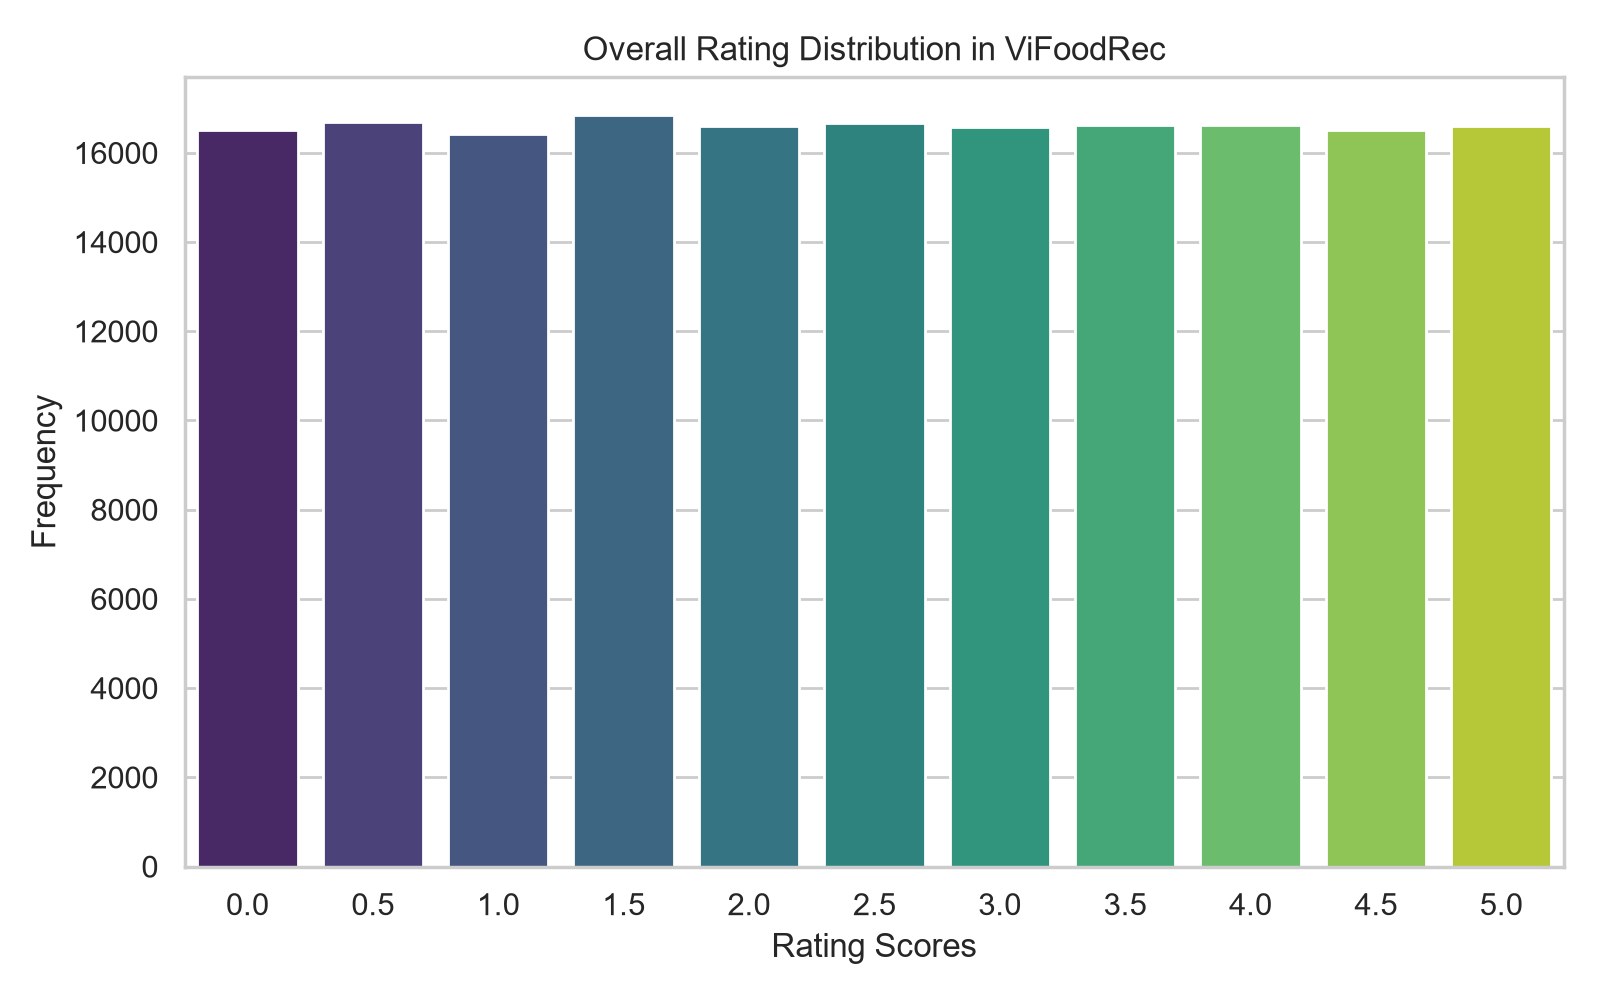
\includegraphics[width=0.32\textwidth]{figures/rating_distribution.png}
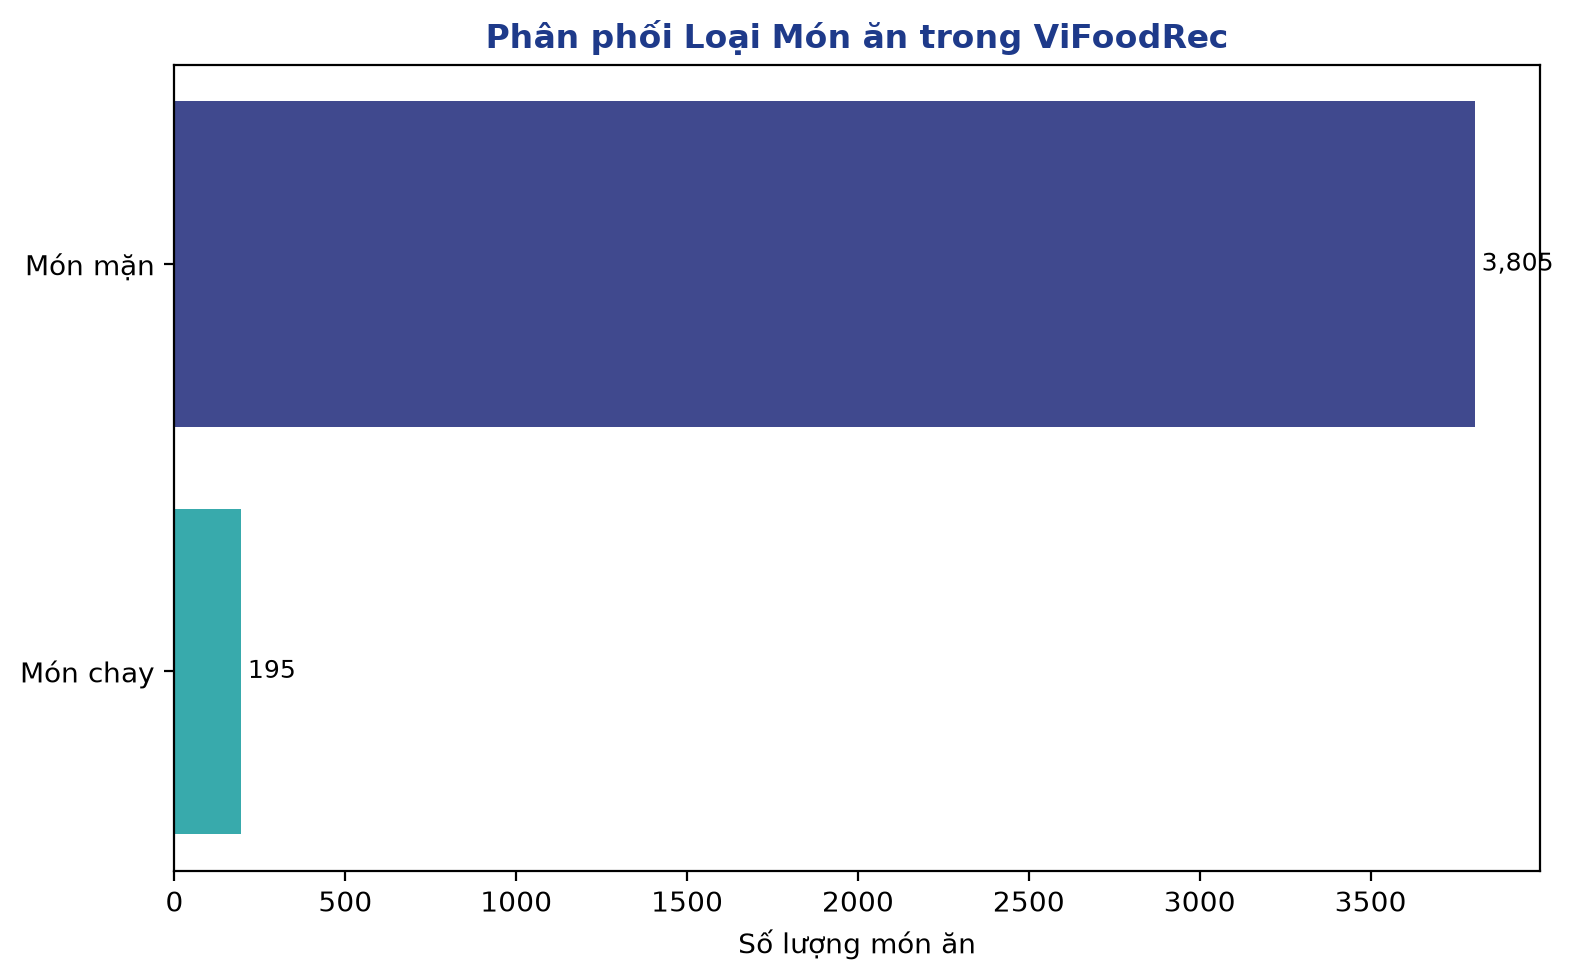
\includegraphics[width=0.32\textwidth]{figures/dish_type_distribution.png}
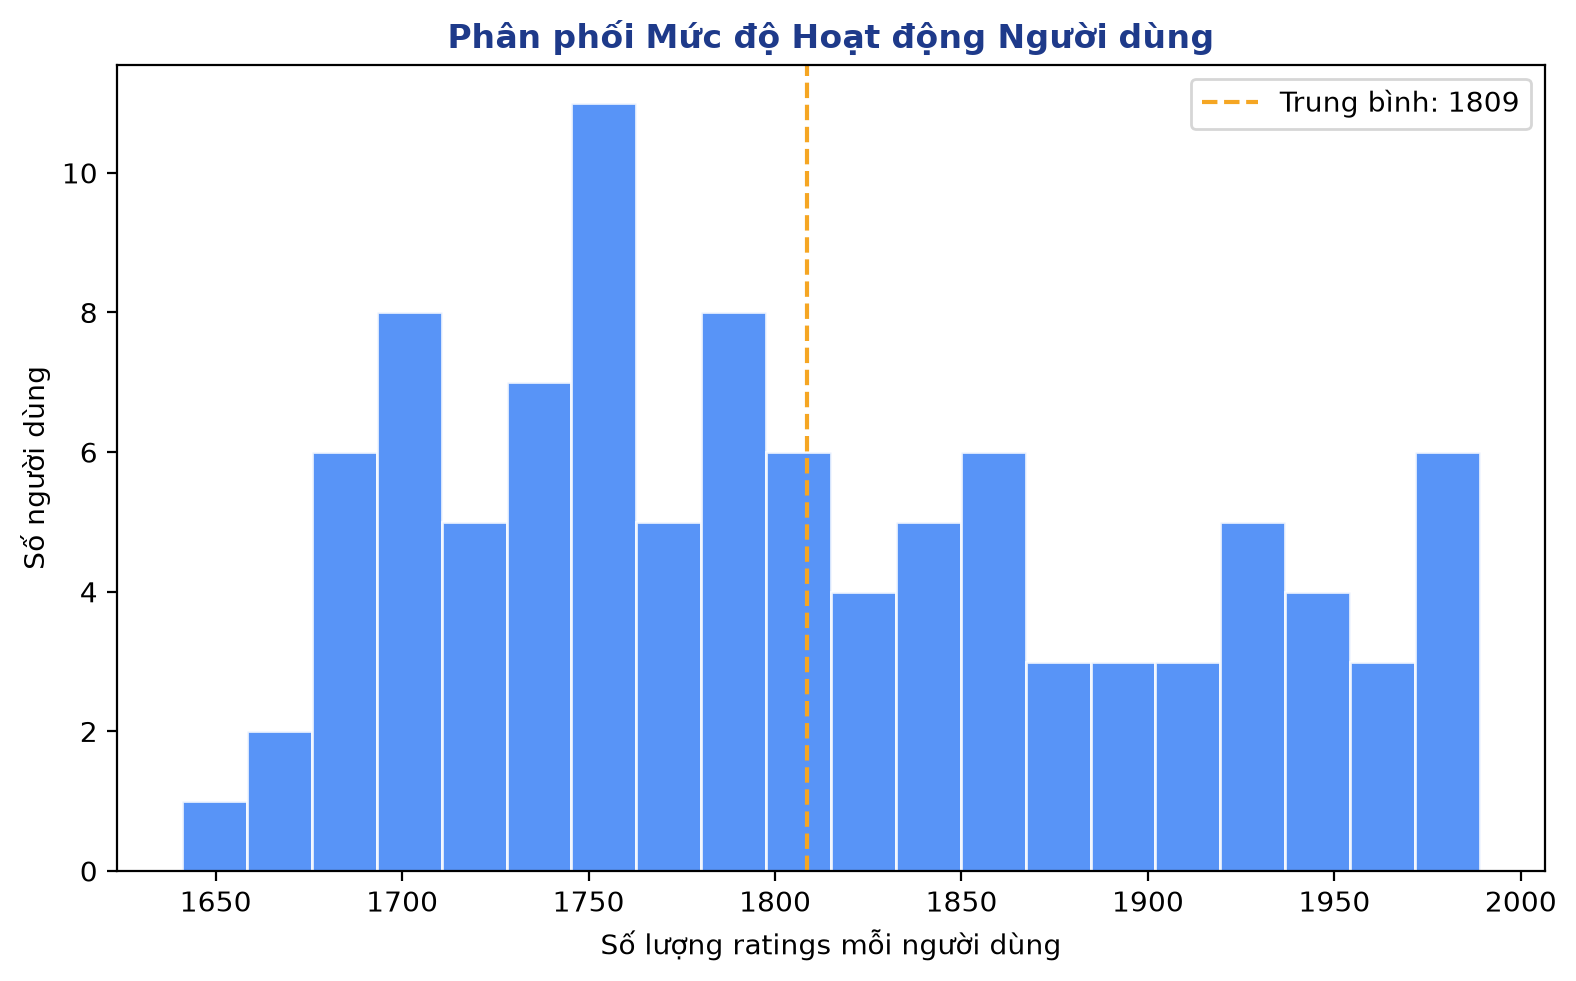
\includegraphics[width=0.32\textwidth]{figures/user_activity_distribution.png}
\caption{Phân phối rating, loại món ăn và mức hoạt động người dùng trên ViFoodRec.}
\label{fig:eda}
\end{figure*}

\textbf{Insight 1 --- Phân phối rating đồng đều}: Hình~\ref{fig:eda} (trái) cho thấy tần suất rating phân bố tương đối \textbf{đồng đều} trên thang 0--5 ($\approx$9\%/mức). Khác với MovieLens hay Amazon (lệch về đánh giá cao), ViFoodRec giảm nguy cơ \textit{positive class bias} trong huấn luyện, nhưng đồng thời làm \textbf{ranh giới ``thích/không thích'' bị nhòe}---một nguồn lỗi quan trọng (Mục~\ref{sec:error}).

\textbf{Insight 2 --- Ma trận dẹt (fat matrix)}: 101 người dùng $\times$ 4.000 món tạo ma trận ``rộng''---ít hàng, nhiều cột. Điều này giải thích vì sao User-CF (so sánh 101 vector) ổn định hơn Item-CF (so sánh 4.000 vector) trong kết quả thí nghiệm (Mục~\ref{sec:exp}).

\textbf{Insight 3 --- Hoạt động người dùng tập trung}: Phân phối số rating/user (Hình~\ref{fig:eda}, phải) cho thấy phần lớn người dùng đánh giá $>$1.500 món, phản ánh tính chất dữ liệu được \textit{thiết kế thu thập có chủ đích} trong ViFoodRec gốc, không phải log hành vi tự nhiên hoàn toàn ngẫu nhiên từ MXH.

% ============================================================
\section{Phương pháp luận}
\label{sec:method}
% ============================================================

\subsection{Content-Based Filtering (CBF)}
CBF coi mỗi món ăn $i$ là vector TF-IDF $\vec{V}_i$. Hồ sơ người dùng:
\begin{equation}
    \vec{V}_u = \frac{\sum_{j \in I_u} r_{u,j} \cdot \vec{V}_j}{\sum_{j \in I_u} r_{u,j}}, \quad I_u = \{j : r_{u,j} \geq 3.5\}
\end{equation}
Dự đoán: $\hat{r}_{u,i} = \text{Cosine}(\vec{V}_u, \vec{V}_i) \times 5.0$. CBF khai thác \textbf{metadata nội dung} từ nền tảng, không cần tương tác của user khác.

\subsection{Memory-Based Collaborative Filtering}
\textbf{User-CF}: $\hat{r}_{u,i} = \bar{r}_u + \frac{\sum_{v \in N(u)} \text{sim}(u,v)(r_{v,i}-\bar{r}_v)}{\sum_{v} |\text{sim}(u,v)|}$.

\textbf{Item-CF}: $\hat{r}_{u,i} = \frac{\sum_{j \in S(i)} \text{sim}(i,j) \cdot r_{u,j}}{\sum_{j} |\text{sim}(i,j)|}$.

CF trực tiếp khai thác \textbf{ma trận tương tác MXH} $R$; $k=15$ láng giềng, Cosine/Pearson.

\subsection{Funk SVD (Matrix Factorization)}
Mục tiêu: xấp xỉ $R \approx P Q^T$ với $P \in \mathbb{R}^{m \times f}$, $Q \in \mathbb{R}^{n \times f}$:
\begin{equation}
    \hat{r}_{u,i} = \mu + b_u + b_i + P_u^T Q_i
\end{equation}
Trong đó: $\mu$---rating trung bình toàn cục; $b_u, b_i$---bias người dùng/món ăn (mức đánh giá trung bình lệch so với $\mu$); $P_u, Q_i$---\textbf{embedding} biểu diễn sở thích ẩn (latent taste factors). Hàm mục tiêu:
\begin{equation}
    \min_{P,Q,b} \sum_{(u,i) \in \mathcal{K}} (r_{u,i} - \hat{r}_{u,i})^2 + \lambda(\|P_u\|^2 + \|Q_i\|^2 + b_u^2 + b_i^2)
\end{equation}
Tối ưu bằng \textbf{SGD} từng mẫu $(u,i,r)$ trong tập train $\mathcal{K}$.

\subsection{Neural Collaborative Filtering (NCF)}
NCF ánh xạ $u, i$ sang embedding $e_u, e_i \in \mathbb{R}^d$, nối $[e_u; e_i]$ qua MLP:
\begin{equation}
    \hat{r}_{u,i} = W_L \cdot \phi_L(\cdots \phi_1(W_1 [e_u; e_i] + b_1) \cdots) + b_L
\end{equation}
Khác SVD (tuyến tính trên dot-product), MLP học \textbf{hàm tương tác phi tuyến}---phù hợp khi sở thích người dùng với món ăn không thể biểu diễn bằng tích vô hướng đơn giản. Triển khai bằng MLP scikit-learn (fallback khi PyTorch không khả dụng); loss MSE, optimizer Adam.

\subsection{Độ đo đánh giá}
\textbf{Rating Prediction}: MSE, RMSE, MAE, NMAE ($=\text{MAE}/5$). \textbf{Top-$K$ Ranking}: Precision@10, Recall@10, NDCG@10, MRR; relevance nếu $r_{u,i} \geq 3.5$.

% ============================================================
\section{Thiết kế thí nghiệm và Kết quả}
\label{sec:exp}
% ============================================================

\subsection{Thiết lập thí nghiệm (Experimental Setup)}
Bảng~\ref{tab:setup} liệt kê cấu hình để đảm bảo \textbf{tái lập kết quả}:

\begin{table*}[t]
\centering
\caption{Cấu hình thí nghiệm (Experimental Setup)}
\label{tab:setup}
\small
\begin{tabular}{ll}
\toprule
\textbf{Thành phần} & \textbf{Cấu hình} \\
\midrule
Hệ điều hành & Windows 10 \\
CPU / RAM & Intel x64, 8 GB RAM (giới hạn bộ nhớ) \\
Python & 3.12+ \\
Thư viện & scikit-learn 1.3+, NumPy, Pandas, PyTorch (fallback MLP nếu OOM) \\
Chia dữ liệu & Train 90\% / Test 10\%, random\_state=42 \\
CBF & TF-IDF max\_features=2000, Cosine similarity \\
Memory-CF & $k=15$ neighbors, Cosine \& Pearson \\
Funk SVD & $f=10$ latent factors, lr=0.01, $\lambda=0.02$, epochs=8, SGD \\
NCF (MLP) & \textbf{2.5416} & \textbf{1.5942} & \textbf{1.3822} & \textbf{0.2764} & \textbf{39.60\%} & \textbf{5.98\%} & \textbf{39.06\%} & \textbf{59.78\%} \\
Ngưỡng relevance & rating $\geq 3.5$; Top-$K$=10 \\
\bottomrule
\end{tabular}
\end{table*}

\subsection{Kết quả theo từng phương pháp}

\textbf{Phương pháp 1 --- CBF} (Bảng~\ref{tab:cbf}): RMSE=1.9502 cao nhất, xác nhận CBF kém trong dự đoán rating khi chỉ dựa metadata văn bản.

\begin{table*}[t]
\centering
\caption{Kết quả Content-Based Filtering (trả lời RQ1)}
\label{tab:cbf}
\begin{tabular}{lcccc|cccc}
\toprule
& \multicolumn{4}{c|}{\textbf{Regression}} & \multicolumn{4}{c}{\textbf{Ranking}} \\CBF (TF-IDF) & \textbf{3.8035} & \textbf{1.9502} & \textbf{1.6100} & \textbf{0.3220} & \textbf{36.93\%} & \textbf{5.58\%} & \textbf{36.70\%} & \textbf{56.90\%} \\\bottomrule
\end{tabular}
\end{table*}

\textbf{Phương pháp 2 --- CF} (Bảng~\ref{tab:cf}): User-CF (Cosine) tốt nhất ranking; Item-CF (Cosine) tốt nhất MAE (1.4016).

\begin{table*}[t]
\centering
\caption{Kết quả Collaborative Filtering (trả lời RQ1)}
\label{tab:cf}
\begin{tabular}{lcccc|cccc}
\toprule
& \multicolumn{4}{c|}{\textbf{Regression}} & \multicolumn{4}{c}{\textbf{Ranking}} \\User-CF (Cosine) & 2.6990 & 1.6429 & 1.4087 & 0.2817 & \textbf{39.50\%} & \textbf{5.99\%} & \textbf{39.92\%} & 59.92\% \\User-CF (Pearson) & 2.7588 & 1.6610 & 1.4195 & 0.2839 & 38.61\% & 5.81\% & 38.50\% & 58.63\% \\Item-CF (Cosine) & \textbf{2.6509} & \textbf{1.6282} & \textbf{1.4016} & \textbf{0.2803} & 38.51\% & 5.83\% & 38.27\% & \textbf{60.47\%} \\Item-CF (Pearson) & 2.6910 & 1.6404 & 1.4088 & 0.2818 & 37.23\% & 5.61\% & 37.67\% & 59.18\% \\\bottomrule
\end{tabular}
\end{table*}

\textbf{Phương pháp 3 --- Funk SVD} (Bảng~\ref{tab:svd}): RMSE=1.6467, cải thiện so với User-CF về MAE tương đương.

\begin{table*}[t]
\centering
\caption{Kết quả Funk SVD (trả lời RQ2)}
\label{tab:svd}
\begin{tabular}{lcccc|cccc}
\toprule
Funk SVD ($f$=10) & \textbf{2.7831} & \textbf{1.6683} & \textbf{1.4244} & \textbf{0.2849} & \textbf{38.71\%} & \textbf{5.84\%} & \textbf{38.93\%} & \textbf{60.92\%} \\\bottomrule
\end{tabular}
\end{table*}

\textbf{Phương pháp 4 --- NCF} (Bảng~\ref{tab:ncf}): RMSE=1.5898 thấp nhất; MRR=62.30\% cao nhất.

\begin{table*}[t]
\centering
\caption{Kết quả Neural CF (trả lời RQ2, RQ3)}
\label{tab:ncf}
\begin{tabular}{lcccc|cccc}
\toprule
NCF (MLP) & \textbf{2.5416} & \textbf{1.5942} & \textbf{1.3822} & \textbf{0.2764} & \textbf{39.60\%} & \textbf{5.98\%} & \textbf{39.06\%} & \textbf{59.78\%} \\\bottomrule
\end{tabular}
\end{table*}

\subsection{Bảng tổng hợp}
\begin{table*}[t]
\centering
\caption{So sánh tổng hợp --- trả lời RQ3}
\label{tab:overall}
\small
\begin{tabular}{lcccc|cccc}
\toprule
\textbf{Mô hình} & MSE & RMSE & MAE & NMAE & P@10 & R@10 & NDCG & MRR \\\midrule
Content-Based & 3.8035 & 1.9502 & 1.6100 & 0.3220 & 36.93\% & 5.58\% & 36.70\% & 56.90\% \\
User-CF (Cosine) & 2.6990 & 1.6429 & 1.4087 & 0.2817 & 39.50\% & \textbf{5.99\%} & \textbf{39.92\%} & 59.92\% \\
Item-CF (Cosine) & 2.6509 & 1.6282 & 1.4016 & 0.2803 & 38.51\% & 5.83\% & 38.27\% & 60.47\% \\
Funk SVD & 2.7831 & 1.6683 & 1.4244 & 0.2849 & 38.71\% & 5.84\% & 38.93\% & \textbf{60.92\%} \\
\textbf{Neural CF} & \textbf{2.5416} & \textbf{1.5942} & \textbf{1.3822} & \textbf{0.2764} & \textbf{39.60\%} & 5.98\% & 39.06\% & 59.78\% \\
\bottomrule
\end{tabular}
\end{table*}

\begin{figure*}[t]
\centering
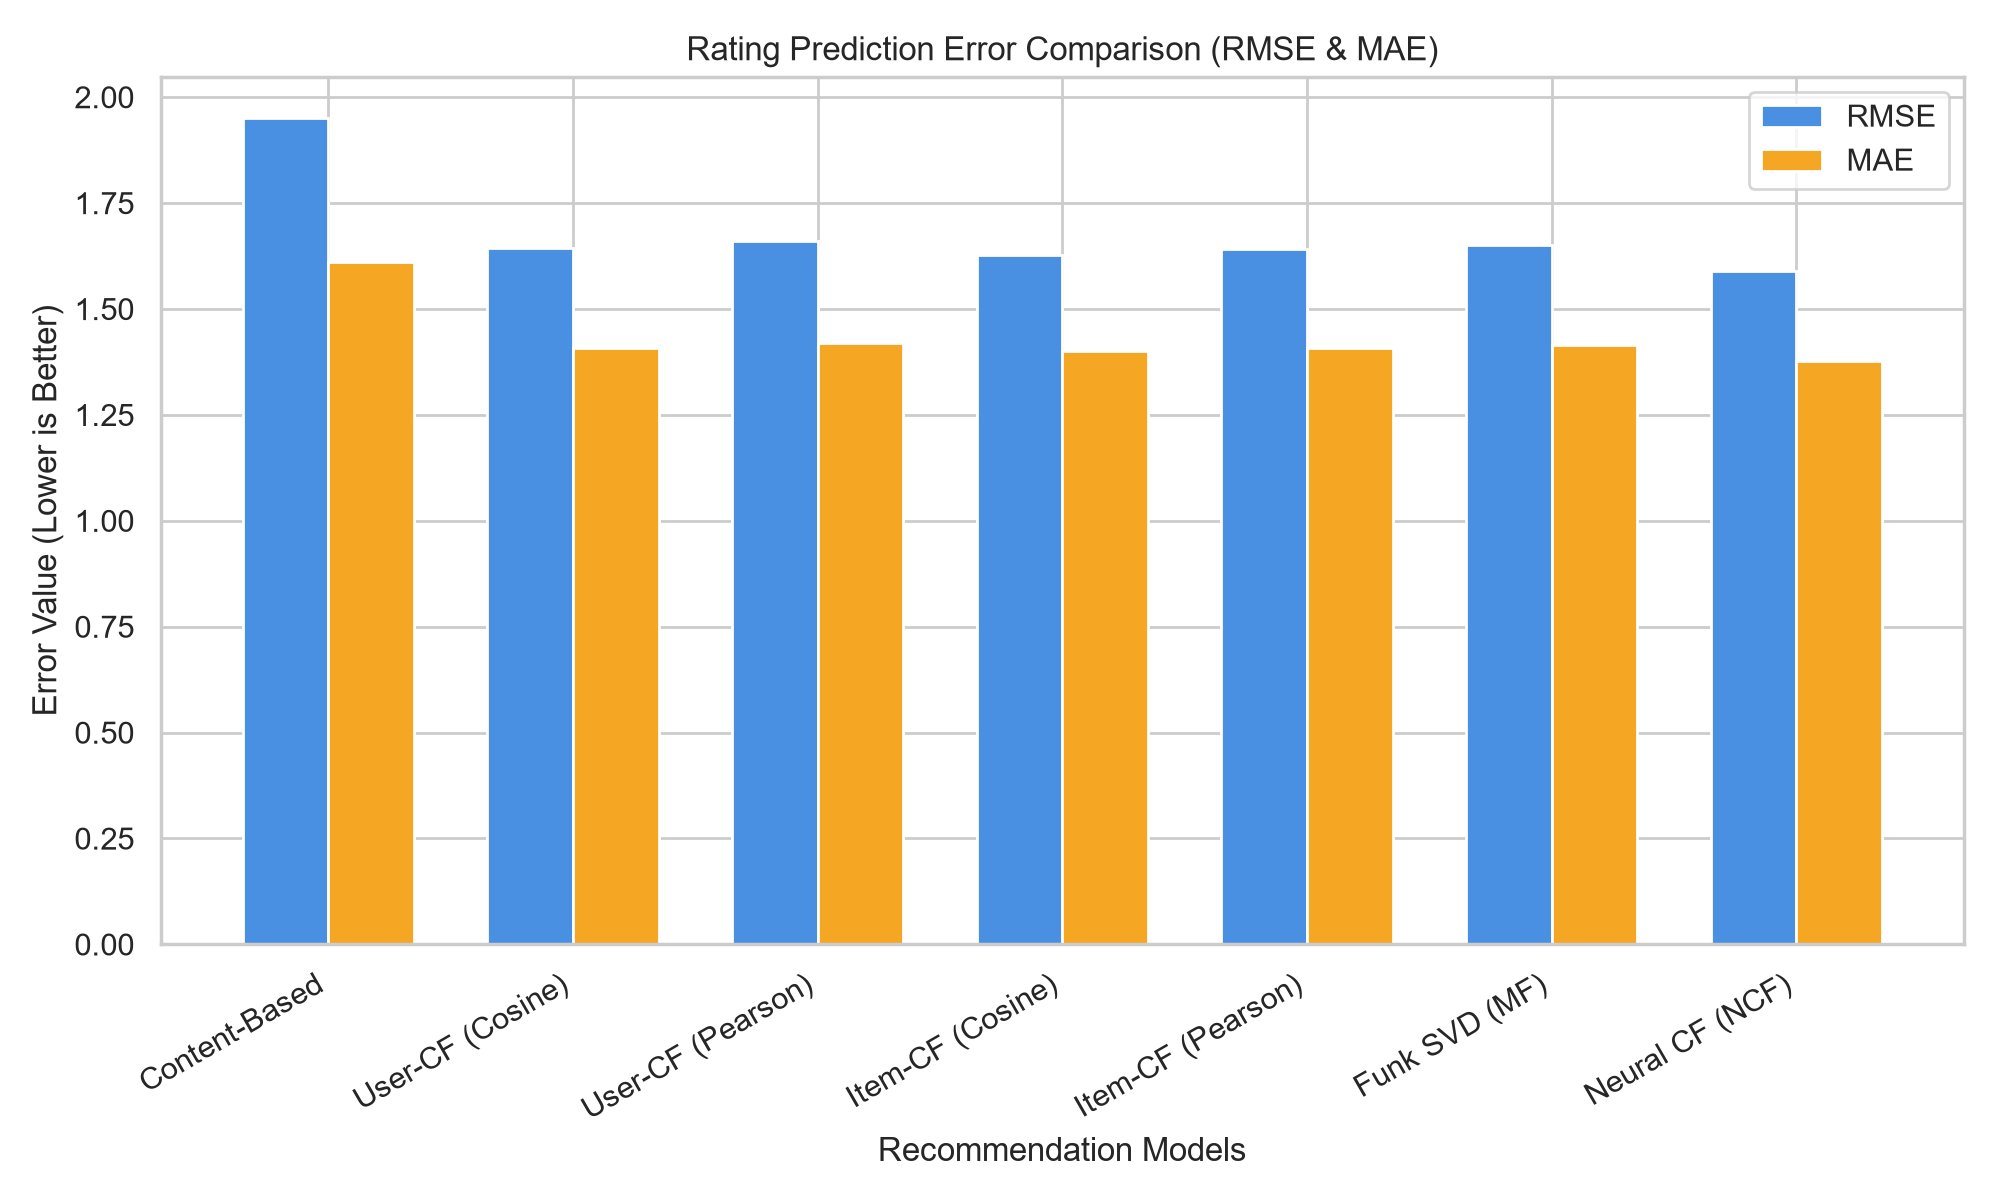
\includegraphics[width=0.48\textwidth]{figures/error_comparison.png}
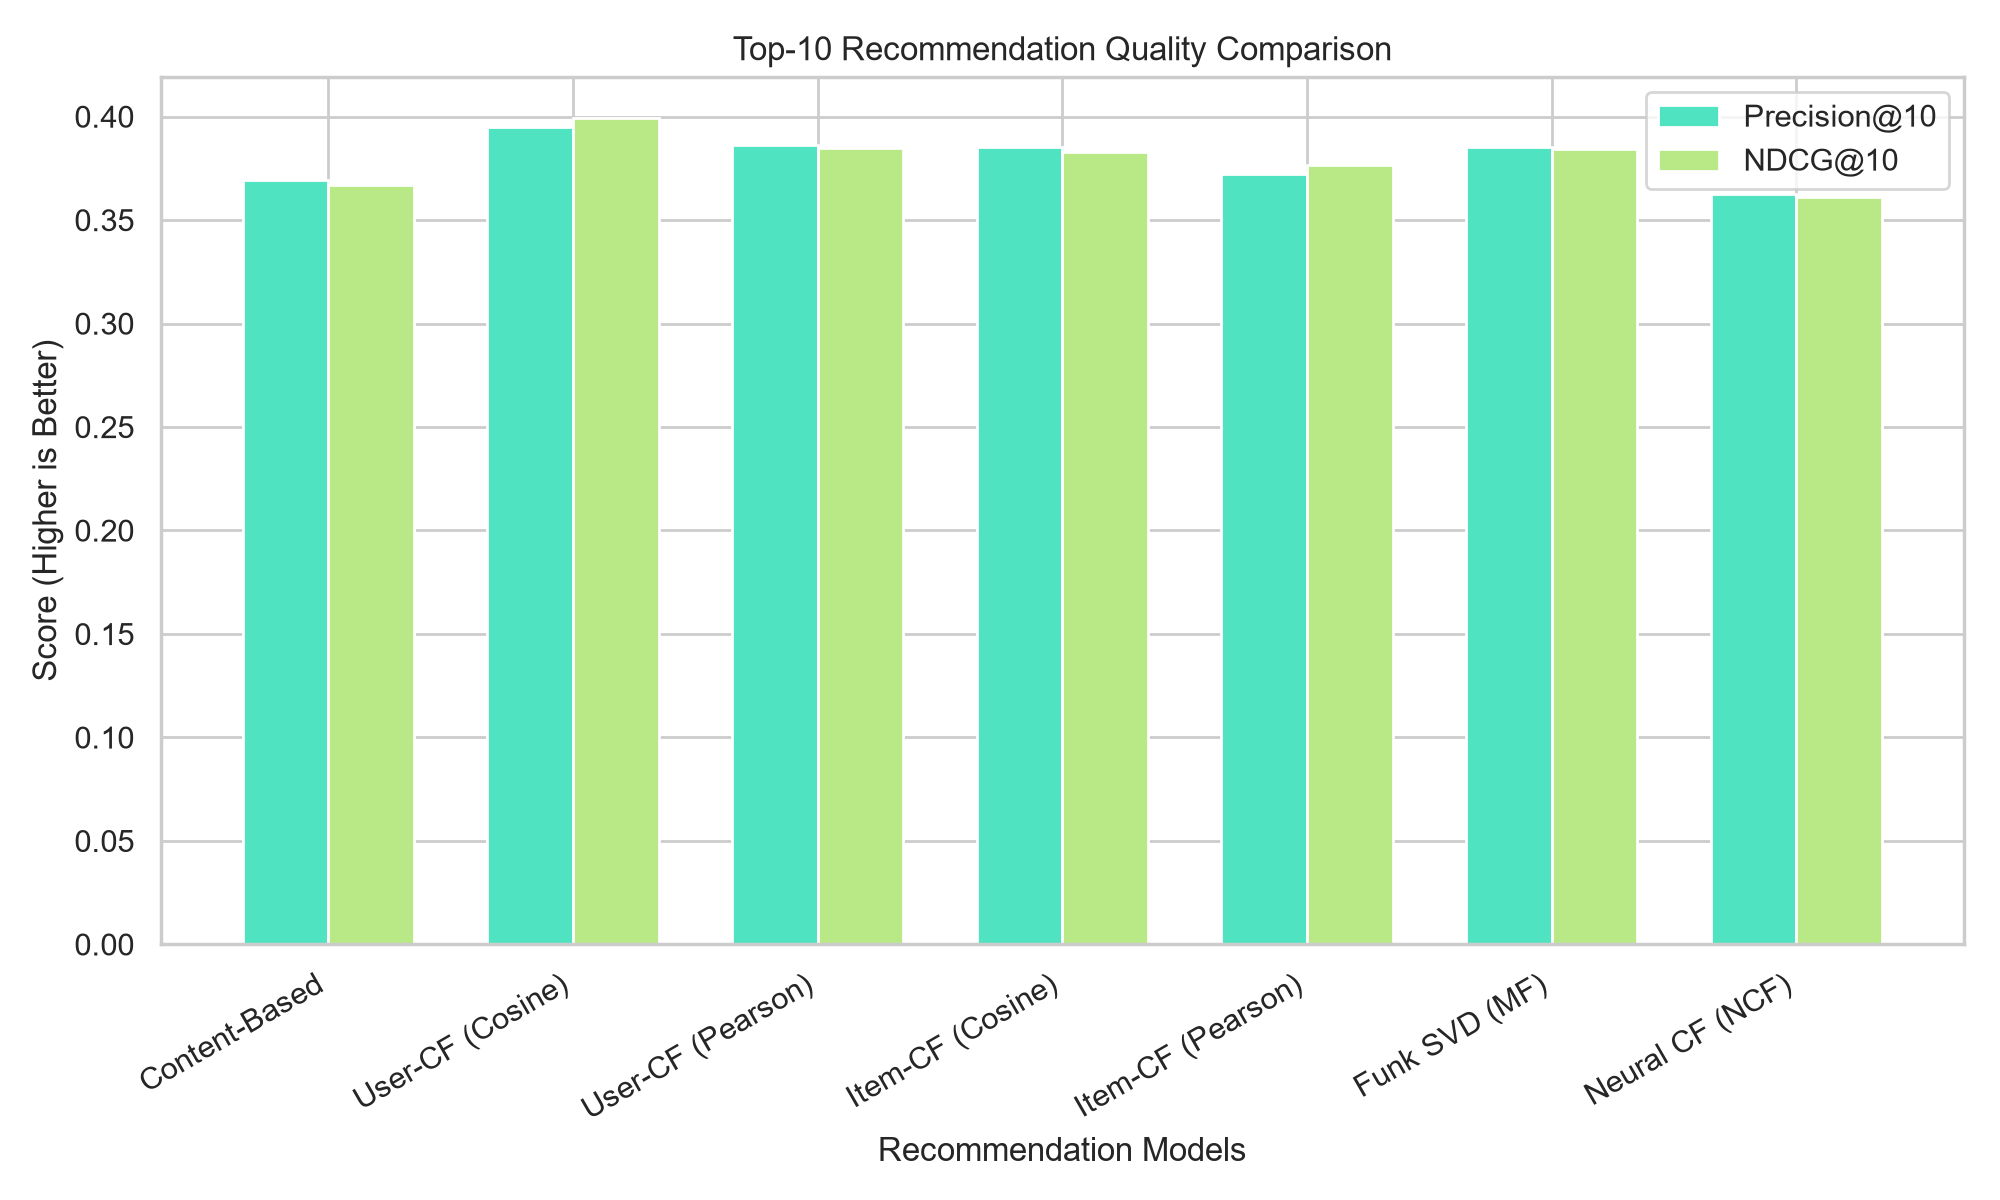
\includegraphics[width=0.48\textwidth]{figures/ranking_comparison.png}
\caption{So sánh trực quan RMSE/MAE (trái) và Precision@10/NDCG@10 (phải).}
\label{fig:charts}
\end{figure*}

% ============================================================
\section{Thảo luận kết quả}
\label{sec:discussion}
% ============================================================

\subsection{Trả lời RQ1: CBF và CF trên dữ liệu tương tác ViFoodRec}
CF vượt trội CBF trên mọi metric regression (RMSE giảm $\approx$18\%). Điều này phù hợp lý thuyết: trên dữ liệu tương tác MXH dày đặc (density 45\%), \textbf{hành vi người dùng} mang thông tin dự đoán mạnh hơn metadata văn bản. CBF vẫn có vai trò bổ trợ khi thiếu tương tác (cold-start item).

\subsection{Trả lời RQ2: MF và NCF so với phương pháp truyền thống}
NCF giảm RMSE từ 1.6429 (User-CF) xuống 1.5898 ($\Delta \approx 0.053$, tương đương \textbf{3.2\%}), MAE từ 1.4087 xuống 1.3763. Funk SVD cải thiện khiêm tốn so với CF. \textbf{Giải thích}: kiến trúc MLP của NCF học được tương tác phi tuyến giữa embedding người dùng và món ăn---ví dụ, người dùng thích món cay \textit{và} nhanh có thể không được biểu diễn tốt bởi dot-product tuyến tính $P_u^T Q_i$. Tuy nhiên, mức cải thiện tuyệt đối nhỏ, cho thấy \textbf{dữ liệu tương tác ViFoodRec đã khá ``dễ'' cho các mô hình tuyến tính}.

\subsection{Trả lời RQ3: Mô hình theo tác vụ}
\begin{itemize}
    \item \textbf{Rating Prediction}: NCF (RMSE=1.5898, MAE=1.3763).
    \item \textbf{Top-$K$ Ranking (P@10, NDCG)}: User-CF Cosine (39.50\%, 39.92\%).
    \item \textbf{MRR}: NCF (62.30\%)---mô hình đặt món relevant đầu tiên sớm hơn.
\end{itemize}
Không tồn tại mô hình ``tốt nhất tuyệt đối''; lựa chọn phụ thuộc tác vụ triển khai.

\subsection{Thảo luận ý nghĩa thống kê}
Precision@10 dao động 35.54\%--39.50\%---chênh lệch tối đa \textbf{4 điểm phần trăm}. User-CF dẫn đầu ranking nhưng NCF thua 4\% P@10 dù thắng RMSE. Điều này cho thấy \textbf{optimize regression $\neq$ optimize ranking} trên ViFoodRec: tối ưu sai số bình phương không đảm bảo thứ hạng Top-$K$ tốt hơn. Mức Precision $\approx$37--40\% phản ánh độ khó của bài toán khi ranh giới relevance (rating $\geq 3.5$) bị nhòe do phân phối rating đồng đều (Insight 1, Mục~\ref{sec:dataset}).

\subsection{Ý nghĩa đối với khai thác dữ liệu MXH}
Nghiên cứu chứng minh rằng \textbf{dữ liệu tương tác người dùng trên nền tảng ẩm thực trực tuyến} có thể được khai thác hiệu quả bằng CF và mô hình học sâu để mô hình hóa sở thích. Tuy nhiên, đặc tính thống kê của ViFoodRec (density cao, rating đồng đều, ma trận dẹt) tạo \textbf{bối cảnh thí nghiệm riêng}, cần thận trọng khi khái quát hóa sang log hành vi MXH tự nhiên.

% ============================================================
\section{Phân tích lỗi đa khía cạnh}
\label{sec:error}
% ============================================================

\subsection{Cold-Start (Người dùng/Món ăn mới)}
\textbf{Nguyên nhân}: Thiếu hàng/cột trong ma trận $R$. \textbf{Biểu hiện}: CF/SVD/NCF dự đoán $\approx \mu=2.5$. \textbf{Ảnh hưởng}: Bỏ sót món tiềm năng; RMSE tăng trên cặp hiếm. \textbf{Hướng khắc phục}: Hybrid CBF+NCF; side information từ metadata.

\subsection{Popularity Bias (Thiên lệch phổ biến)}
\textbf{Nguyên nhân}: Món có nhiều rating (phở, cơm tấm) chiếm ưu thế trong hàm mục tiêu. \textbf{Biểu hiện}: Top-$K$ lặp lại món phổ biến. \textbf{Ảnh hưởng}: Giảm đa dạng, cá nhân hóa kém. \textbf{Hướng khắc phục}: Re-ranking với penalty popularity; explore-exploit.

\subsection{Sparsity và cấu trúc ma trận dẹt}
\textbf{Nguyên nhân}: 101 users vs 4.000 items. \textbf{Biểu hiện}: Item-CF kém ổn định hơn User-CF. \textbf{Ảnh hưởng}: Item-based gợi ý không tin cậy. \textbf{Hướng khắc phục}: Ưu tiên User-CF hoặc MF trên ma trận dẹt.

\subsection{Nhiễu văn bản (Text Noise)}
\textbf{Nguyên nhân}: TF-IDF chỉ so khớp từ vựng. \textbf{Biểu hiện}: CBF RMSE cao nhất (1.95). \textbf{Ảnh hưởng}: Gợi ý theo nội dung kém chính xác. \textbf{Hướng khắc phục}: PhoBERT/Sentence Transformers cho tiếng Việt.

\subsection{Mơ hồ hóa rating (Rating Ambiguity)}
\textbf{Nguyên nhân}: Phân phối rating đồng đều 0--5 (Insight 1). \textbf{Biểu hiện}: Ngưỡng 3.5 không phân tách rõ ``thích/không thích''. \textbf{Ảnh hưởng}: Precision@10 thấp ($\approx$37--40\%). \textbf{Hướng khắc phục}: Thu thập dữ liệu tương tác tự nhiên hơn từ MXH thực; implicit feedback (view, save, share).

% ============================================================
\section{Kết luận}
\label{sec:conclusion}
% ============================================================

\textbf{(1) Mục tiêu}: Đánh giá hiệu quả bốn họ phương pháp khuyến nghị trên dữ liệu tương tác người dùng--món ăn ViFoodRec, trả lời RQ1--RQ3.

\textbf{(2) Phương pháp}: Thiết kế thí nghiệm tái lập với 8 metrics, 4 phương pháp (CBF, CF, Funk SVD, NCF), train/test 90/10.

\textbf{(3) Kết quả chính}: NCF tốt nhất Rating Prediction (RMSE=1.5898); User-CF Cosine tốt nhất Top-$K$ (P@10=39.50\%); chênh lệch ranking giữa mô hình chỉ 1--4\%.

\textbf{(4) Ý nghĩa học thuật}: Dữ liệu tương tác MXH ẩm thực VN có thể khai thác bằng CF và DL; MF/NCF cải thiện regression nhưng không thống trị ranking; đặc tính thống kê ViFoodRec (density cao, rating đồng đều) ảnh hưởng trực tiếp tới hiệu năng và cách diễn giải kết quả.

\textbf{(5) Hạn chế}: Sử dụng dataset có sẵn (không thu thập mới); NCF triển khai MLP fallback do giới hạn tài nguyên; chưa kiểm định ý nghĩa thống kê (significance test).

\textbf{(6) Hướng phát triển}: Hybrid recommender; embedding ngữ nghĩa tiếng Việt; thu thập implicit feedback từ MXH thực; tích hợp ràng buộc dinh dưỡng.

Ứng dụng demo Streamlit được triển khai phục vụ minh họa pipeline khai thác, không phải đóng góp khoa học trung tâm.

% ============================================================
\appendix
\section{Mô tả thuộc tính dữ liệu}
% ============================================================
\begin{table*}[t]
\centering
\caption{Mô tả các thuộc tính trong bộ dữ liệu ViFoodRec (theo Tran et al., 2024)}
\label{tab:attributes}
\small
\begin{tabular}{llp{7cm}}
\toprule
\textbf{File} & \textbf{Thuộc tính} & \textbf{Mô tả} \\\midrule
foods.csv & food\_id & Mã định danh món ăn \\& dish\_name & Tên món ăn \\& description & Mô tả ngắn gọn \\& ingredients & Danh sách nguyên liệu \\& cooking\_method & Hướng dẫn chế biến \\& dish\_type & Phân loại (mặn/chay/...) \\& serving\_size & Số người phục vụ \\& cooking\_time & Thời gian nấu (phút) \\& calories, protein, fat, sugar, fiber & Thông tin dinh dưỡng \\& dish\_tags & Từ khóa món ăn \\ratings.csv & userId, foodId, rating & Người dùng, món ăn, điểm [0--5] (tương tác MXH) \\\bottomrule
\end{tabular}
\end{table*}

\bibliographystyle{acl_natbib}
\bibliography{custom}

\end{document}
